%%%%%%%%%%%%%%%%%%%%%%%%%%%%%%%%%%%%%%%%%%%%%%%%%%%%%%%%%%%%%%%%%%%%%%%%%%%%%%%
%% StuPro B, "Programmierumgebung Offener Antrieb" (POA)
%% Entwurf
%% $Id: xmldoku.tex,v 1.1 2004/05/18 23:51:49 vanto Exp $
%%%%%%%%%%%%%%%%%%%%%%%%%%%%%%%%%%%%%%%%%%%%%%%%%%%%%%%%%%%%%%%%%%%%%%%%%%%%%%%
\documentclass[a4paper,titlepage,12pt,ngerman]{scrbook}
\usepackage{../common/header}

\RCSdef $Revision: 1.1 $
\RCSdef $Date: 2004/05/18 23:51:49 $

\newcommand\version{Version \today \xspace}
%\newcommand\version{Version 1.0\xspace}

\title {\huge \product\\[0.5cm]\large Entwurf\\[0.5cm] \version
  \\[1cm] \Large \company}

\begin{document}

%%%%%%%%%%%%%%%%%%%%%%%%%%%%%%%%%%%%%%%%%%%%%%%%%%%%%%%%%%%%%%%%%%%%%%%%%%%%%%%
%% Deckblatt

\begin{titlepage}
\renewcommand{\thefootnote}{\fnsymbol{footnote}}
{\Huge
\raggedright
\textbf{POA} \\
\huge Programmierumgebung Offener Antrieb
\rule{\textwidth}{0.75pt}
\par
}
\begin{flushleft}
\normalsize
\version
\end{flushleft}
\vfill

{\parindent=0cm
\Huge POA Projekt-Dateiformat
}


\setcounter{footnote}{0}
\end{titlepage}

%%%%%%%%%%%%%%%%%%%%%%%%%%%%%%%%%%%%%%%%%%%%%%%%%%%%%%%%%%%%%%%%%%%%%%%%%%%%%%%
%% Versionsgeschichte

\section*{Versionsgeschichte}

\begin{itemize}

\item Version 1.0 (1.4.2003)

  Diese Version wurde dem Auftraggeber vorgelegt.

\end{itemize}

%%%%%%%%%%%%%%%%%%%%%%%%%%%%%%%%%%%%%%%%%%%%%%%%%%%%%%%%%%%%%%%%%%%%%%%%%%%%%%%
%% Inhaltsverzeichnis

\tableofcontents

%%%%%%%%%%%%%%%%%%%%%%%%%%%%%%%%%%%%%%%%%%%%%%%%%%%%%%%%%%%%%%%%%%%%%%%%%%%%%%%
%% Format
%%%%%%%%%%%%%%%%%%%%%%%%%%%%%%%%%%%%%%%%%%%%%%%%%%%%%%%%%%%%%%%%%%%%%%%%%%%%%%%
%% StuPro B, "Programmierumgebung Offener Antrieb" (POA)
%% Entwurf
%% $Id: format.tex,v 1.1 2004/05/18 23:51:49 vanto Exp $
%% Achtung: Diese Datei wird in den Entwurf inkludiert!
%%%%%%%%%%%%%%%%%%%%%%%%%%%%%%%%%%%%%%%%%%%%%%%%%%%%%%%%%%%%%%%%%%%%%%%%%%%%%%%

\chapter {Einleitung}
Dieses Dokument beschreibt das Format der POA Projektdateien. Diese
Dateien werden im XML-Format im Projektverzeichnis abgelegt.

Die Datei gliedert sich auf h�chster Ebene in zwei Teile, die von dem
Wurzelelement umschlossen werden. Der erste Teile repr�sentiert das
Datenmodell, der zweite Teil bezieht sich auf die Darstellung der
Bl�cke. Diese View-Elemente beziehen sich �ber eine ID auf den
jeweiligen Block im Modell-Bereich. Eine Ausnahme bilden hier die
Verbindungen zwischen Bl�cken. Diese haben keine Modellinstanz sondern
werden nur als View-Element abgespeichert.

Die folgende Abbildung verdeutlicht den Aufbau der Projektdatei.

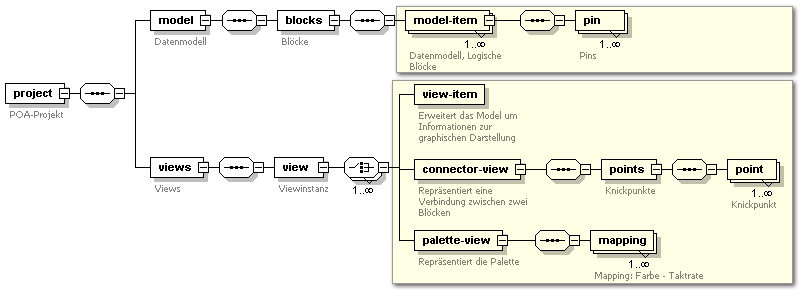
\includegraphics[width=16cm]{poa-schema}

\chapter{Struktur}
%TODO: weird table stuff

\chapter{Daten}
%TODO: weird table stuff

\chapter{Anhang A - DTD}
\chapter{Anhang B - XSD}

%%% Local Variables: 
%%% TeX-master: "xmldoku"
%%% End: 
%%% vim:tw=79:


\end{document}
%%% vim:tw=79:
